%Tex spell check = en-US

%------------------------------------------------------------------------------------
%	PACKAGES AND OTHER DOCUMENT CONFIGURATIONS
%------------------------------------------------------------------------------------
\documentclass[12pt,a4paper]{article}
\input{structure.tex} % Include the file specifying the document structure and custom commands


\newlength{\storeparskip}
\setlength{\storeparskip}{\parskip}

\setlength{\parskip}{\baselineskip}%
\setlength{\parindent}{0pt}%


%-------------------- VARS ----------------------
\newcommand{\authorName}{Gilles Callebaut}
\newcommand{\dateSessionOne}{22/02/2019 13h30\ -\ 16h30}
\newcommand{\dateSessionTwo}{08/03/2019 13h30\ -\ 16h30}
\newcommand{\dateSessionThree}{22/03/2019 13h30\ -\ 16h30}
\newcommand{\softDeadline}{04/04/2019\ -\ 20h00}

\title{Lab Assignment --\ Data Transmission\\\vspace{0.5cm}{\Large Multimedia Networks}}
\author{\authorName}

\begin{document}

\maketitle
\vfill


\begin{center}

  \begin{minipage}{0.65\linewidth}
\begin{description}[style=multiline, leftmargin=4cm]
	\item[Lab session 1] \dateSessionOne
	\item[Lab session 2] \dateSessionTwo
	\item[Lab session 3] \dateSessionThree
\end{description}
\vfill
\begin{description}[style=multiline, leftmargin=4cm]
	\item[Deadline] \softDeadline
\end{description}
\vfill
{\footnotesize
This document is subjected to change, please consult the most recent version at: \url{https://github.com/GillesC/Data-Transmission---Multimedia-Networks}.
}
\end{minipage}
\end{center}

\vfill
\clearpage


%------------------------------------------------------------------------------------
%	INTRODUCTION
%------------------------------------------------------------------------------------
\section{Introduction}
Claude Shannon, an engineer at Bell Telephone Laboratories, and Warren Weaver sought to identify the quickest and most efficient way to get a message from one point to another. As a result of their studies, they developed their model of communication.

In these \textbf{three lab sessions} you are going to simulate a \textbf{communication model} as presented in Figure~\vref{fig:labo1multimedianetwerkendatatransmissiediagram}. This model is a simplified version of the Shannon-Weaver model of communication. The model will be implemented via \textbf{Python}. Through this model, the beneficial effects of source and channel coding are studied. 

\begin{figure}[h]
	\centering
	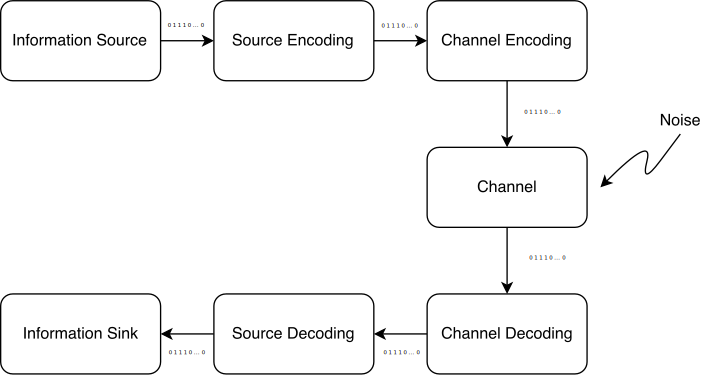
\includegraphics[width=0.7\linewidth]{labo_1_multimedianetwerken_datatransmissie_diagram.pdf}
	\caption{Simplified Model of Communication}\label{fig:labo1multimedianetwerkendatatransmissiediagram}
\end{figure}


\section{Communication Model}
An \textbf{image} will serve as the \textbf{information source}. 
%Encoding and decoding data is computation intensive. Therefore, choosing a small image (e.g.,~40$\times$40) is strongly advised. 
To facilitate interoperability between the communication blocks, we suggest using a \textbf{bit stream} or a \textbf{byte stream} to \textbf{exchange} data between these blocks, i.e.\ every block will receive and send a bit or byte stream to the next one. %The MATLAB template will, by default, use bit streams while the Python template uses \texttt{uint\_8} (byte) streams.

A Python template --and additional library functions-- can be found in the the following Github repository: \url{https://github.com/GillesC/Communication-Model-Python}. How to install the Python environment and the template code is discussed in the Appendix.

\subsection{Source Encoding and Decoding}
Use \textbf{Huffman} and \textbf{Lempel-Ziv-Welch} as a \textbf{source encoding} mechanism. Prior to using the provided template code, study the Huffman and Lempel-Ziv-Welch algorithm. 


\begin{question}
	What is the purpose of source encoding? Try to find an example of a real-life scenario where the effect of absence of source encoding would be clearly noticable.
\end{question}

\begin{question}
	Why does the Lempel-Ziv-Welch Algorithm not group the first occurences of symbols when a combination of the symbols is present in the dictonary?
\end{question}

\begin{question}
	What are the disadvantages of Huffman coding with respect to LZW-coding?
\end{question}

\begin{question}
	What is the correlation between entropy and the number of bits per symbol? 
\end{question}



\subsection{Channel Encoding and Decoding}
\textbf{Reed-Solomon} (RS) coding will be used for \textbf{channel encoding}. 
In this assignment modulation and channel characteristics can be neglected.
After applying Reed-Solomon encoding, 
\begin{itemize}
	\item Simulate storing to disk
	\item Hence, simulate bit errors (with defined error rate)
	\item check if Reed-Solomon is able to resolve the introduced errors and compare with the theoretical limit (Singleton bound).
	\item burst errors
	\item errasures
\end{itemize}

\begin{question}
	Experiment with the code-word length of an RS message, and conclude.%
\end{question}

\begin{question}
	Calculate the number of resolved and unrecoverable errors after introducing the bit errors and or errasures.
\end{question}
 

\section{Objectives}
\begin{itemize}
	\item Build data transmission blocks via Python.%
	\item Enable and disable blocks to determine their impact on the model.%
	\item Measure the transmitted bit stream size of each block and conclude.
	\item Measure the operation duration of each block and conclude.
	For instance, why is Huffman decoding slower than Huffman encoding?
\end{itemize}

\section{Report}
Each student writes an \textbf{individual report}. This report must contain the \textbf{realization} of the aforementioned \textbf{objectives}. It must \textbf{demonstrate} that the student has \textbf{understood} the \textbf{communication model}. 

All Python \textbf{code} must be well \textbf{documented}.
The report and the code has to be send to \texttt{gilles.callebaut@kuleuven.be} and a printed version needs to be handed in. The \textbf{code} itself does \textbf{not} need to be \textbf{included and discussed} in the \textbf{report}. 
The report is expected to be structured and styled as described in~\cite{hoogenboom2012write,kallestinova2011write}.

The report needs to be \textbf{submitted} before \softDeadline.

\begin{description}
	\item[File name format]  \texttt{<firstname>\_<lastname>\_MMN\_report.pdf}
	\item[Language] Dutch or English (recommended)
	\item[Number of pages] Write your report in a compact but concise way, following the
	strategies presented in~\cite{hoogenboom2012write,kallestinova2011write}.
\end{description}

\cleardoublepage%
\appendix
\section{Install Python Environment and Template Code}
\begin{itemize}
	\item Install \href{https://www.anaconda.com/distribution/#download-section}{Anaconda 3} (Python 3.X)
	\item Install Visual Studio Code (default when installing Anaconda) or your favorite edittor/IDE (e.g., PyCharm and Thonny IDE)
	\item Download the template code from Github: \url{https://github.com/GillesC/Communication-Model-Python}.
	\item Install the packages through: \texttt{conda install --file requirements.txt} (in the project folder).
\end{itemize}




\bibliographystyle{plain}
\bibliography{bib}
\end{document}
